% Indicate the main file. Must go at the beginning of the file.
% !TEX root = ../main.tex

%%%%%%%%%%%%%%%%%%%%%%%%%%%%%%%%%%%%%%%%%%%%%%%%%%%%%%%%%%%%%%%%%%%%%%%%%%%%%%%%
% 02_methods
%%%%%%%%%%%%%%%%%%%%%%%%%%%%%%%%%%%%%%%%%%%%%%%%%%%%%%%%%%%%%%%%%%%%%%%%%%%%%%%%

\section{Methods}
\label{methods}

    \subsection{Dataset}

    As part of the Wildlife@Campus project, a labeled dataset was created to train a deep learning algorithm
    The information about the dataset is derived from the dataset itself and a progress report available on GitHub \autocite{ratnaweeraWildlifeCampusProgressReports2021}.
    This dataset is divided into seven sessions --- indicating the source of the images --- the sessions and their origin are listed in \autoref{tab:session_info}.
    The dataset provides two kinds of labels: the original annotations from each session, and a standardized version created when the sessions were integrated into the dataset.
    For this project, only the standardized labels where used.
    Images group into sequences, with each sequence representing a single animal sighting.
    The sequences where created by the Wildlife@Campus team, utilizing the EXIF information of the images to group them based on the time and date of the capture.
    Sequence lengths are not of a fixed length --- the distribution of sequence lengths is shown in \autoref{fig:seq_len_histograms}.
    To get an overview of the available sequences per label, refere to \autoref{fig:sequenceperlabel}.
    The category \texttt{other} represents sequences containing more than one species, this is a result of the process creating the sequences.
    Furthermore, the category \texttt{NaN} represents sequences not labeled --- both where excluded from the from the dataset.
    The category \texttt{glis\_glis} is represented in only four sequences, which is simply not enough to actually train a model to detect it.
    For this reason, it was excluded from the dataset as well.
    This leaves four categories for the classification task: \texttt{apodemus\_sp}, \texttt{cricetidae}, \texttt{soricidae}, and \texttt{mustela\_erminea}.

    %==== table: overview_dataset ====%
    \begin{table}[H]
\caption{Information about the origin of the different sessions in the dataset.}
\label{tab:session_info}
\begin{tabular}{c p{12cm}}
\toprule
Session & Description \\
\midrule
1 & Data from 'the wild', collected durch Wiesel\&Co 2019 \\
2 & Data from 'the wild', collected during WILMA (SummerSchool) 2020 \\
3 & Data from 'the wild', collected by Vogelwarte 2020 \\
4 & Data from 'the wild', collected by WILMA (Bachelorthesis) 2020 \\
5 & Data from 'the wild', collected by WILMA (Roland) 2020 (Contains images and videos of stoats (Mustela erminea)) \\
6 & Data from an enclosure, collected by Nils (Contains only images of stoats (Mustela erminea)) \\
7 & Data gathered from Nathalie Straub in her Bachelor Thesis \\
\bottomrule
\end{tabular}
\end{table}

    %=================================%

    \begin{figure}[H]
    \centering
    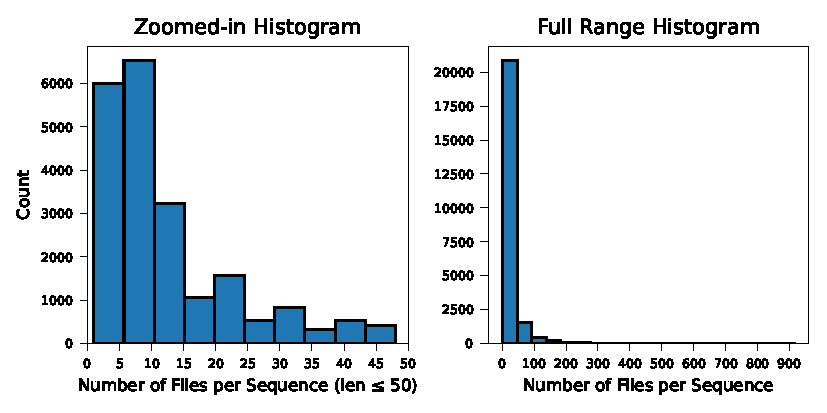
\includegraphics{figures/seq_len_histograms.pdf}
    \caption{Distribution of sequence lengths per label. More than 90\% of the sequences are between 1 and 50 images long. There are longer ones up to a length of 915 images, but these are outliers.}
    \label{fig:seq_len_histograms}
    \end{figure}

    \begin{figure}[H]
    \centering
    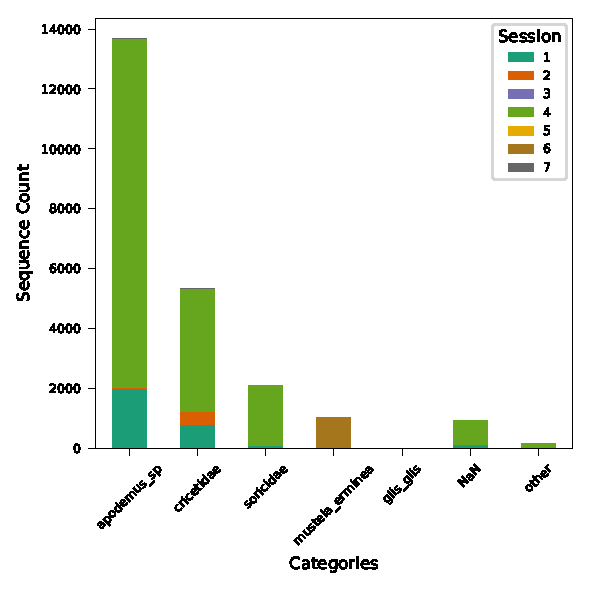
\includegraphics{figures/label2_session.pdf}
    \caption{Available sequences per label colored by session.}
    \label{fig:sequenceperlabel}
    \end{figure}

    \subsection{Data Processing}\todo{create process flow diagram}

    The data processing is divided into tree main steps: Detection, Selection, and Image Processing. 
    Further more a custom data splitting was implemented to create five stratified folds for cross-validation.
    While the detection was performed once for the whole dataset, the selection, image processing, and data splitting were implemented to be done on the fly.

        \subsubsection{Detection and Selection}\todo{Is this okay?}
    
        In this project, the Megadetector (MD) \autocite{morrisEfficientPipelineCamera2025} is used to identify regions of interest (ROI) on all the images.
        The MD outputs a list of bounding boxe (BBox) for detected objects labeled \textit{animal}, \textit{human} or \textit{vehicle} with a corresponding confidence value.
        Only BBoxes with a confidence score above \(0.25\) where storred for further processing.
        This detection step was done sequence wise and the outputs were saved to json files for each sequence.
        An example of how this detections look like is shown in \autoref{fig:detection_example}.
        Only images with a detection labeled \textit{animal} and a confidence score above a certain threshold were retained.  
        The percentage of images discarded per category due to this threshold was determined by inspecting Figure \autoref{fig:lost_images}.  
        In order to reduce noise in the data and eliminate blank inputs to the model, a threshold of \(0.5\) was chosen.
        The trade of was to discard around \(20\%\) of the images for the \textit{soricidae} and \textit{mustela\_erminea} categories.
        For images with multiple detections, only the bounding box with the highest confidence score was kept.

        \begin{figure}[]
        \centering
        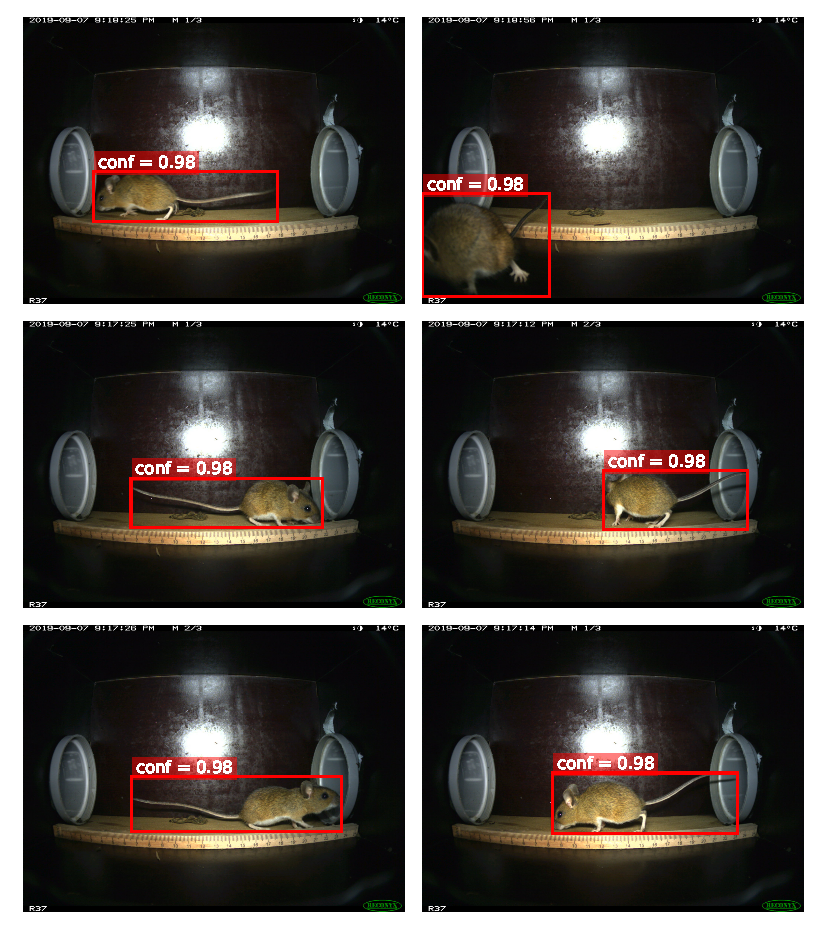
\includegraphics{figures/detections_on_a_sequence.pdf}
        \caption{Example of how the detections look like. The bounding boxes are the six highest confidence detections for the sequence 1001824 a sample from the \textit{apodemus\_sp} category.}
        \label{fig:detection_example}
        \end{figure}

        \begin{figure}[ht]
        \centering
        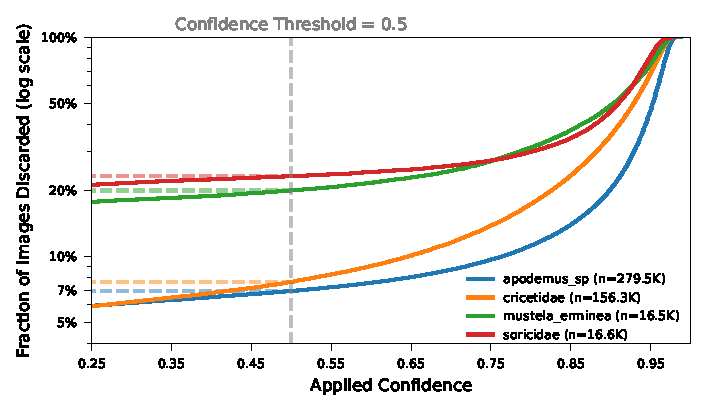
\includegraphics{figures/discarded_img_by_conf.pdf}
        \caption{Fraction of images discarded per category for a detection confidence threshold of 0.5.}
        \label{fig:lost_images}
        \end{figure}        

        \subsubsection{Image Processing}
        To process the images a custom transformation pipline was implemented using transform version 2 from the torchvision library and a custom crop function.
        This transformation was applied on the fly by the PyTorch DataLoader.
        Cropping was done using the BBoxes from the MD detection extending the BBox in order to cut the ratio expected by the model.
        In the case that the extended BBox surpasses the image border the image was padded with black pixels.
        After cropping, each image was resized to the model's expected input size, i.e. \(224\times224\) pixels.
        Each image was first converted into a tensor of shape \((C,H,W)\). 
        The pixel values were then normalized using the global channel wise mean and standard deviation of the dataset itself.
        This mean and standard deviation were calculated on the whole dataset, not just the training set, to ensure consistency across all folds.
        Furthermore, only the best BBox area per image was used to calculate the mean and standard deviation.

        \subsubsection{Data Splitting}
        The dataset was split into five folds using a stratified split based on the classes.
        A custom helper function was implemented to ensure the splits are done on a sequence level, meaning no sequence is ever split between folds.
        The fold size was determined by the number of images instead of the number of sequences, as the sequences vary in length.
        This approach ensures that the images are evenly distributed across the folds while maintaining the sequence integrity.
        For each class in the dataset, all the sequences were shuffled using a fixed seed for reproducibility resulting in two lists: one with the sequence ids and one with the corresponding sequence lengths.
        The list with sequence lengths was used to determine the cut-points for the folds while the list with sequence ids was used to assign the sequences to the folds.


    \subsection{Model}

    In this project, a selection of models from the torchvision library was tested to classify the images. 
    Every model was both trained from scratch and fine-tuned using the weights of a model pre-trained on ImageNet \autocite{dengImageNetLargescaleHierarchical2009}.
    A custom helper function was implemented to adapt the last layer of the model to fit the number of classes in the dataset when the model is loaded.
    The models used in this project are:

    \begin{itemize}
        \item \textbf{EfficientNet-B0} \autocite{tanEfficientNetRethinkingModel2019}:  
        A Convolutional Neural Network architecture that uses a compound scaling method to uniformly scale network width, depth, and resolution.  
        The B0 variant is the baseline model from which larger EfficientNets are derived.  

        \item \textbf{DenseNet-169} \autocite{huangDenselyConnectedConvolutional2017}:  
        A densely connected convolutional network with 169 layers in which each layer receives feature-maps from all preceding layers, fostering feature reuse and improved gradient flow.  

        \item \textbf{ResNet-50} \autocite{heDeepResidualLearning2016}:  
        A 50-layer Residual Network that introduces skip connections (residual blocks) to alleviate the vanishing-gradient problem, enabling training of very deep models.  

        \item \textbf{ViT-B\_16} \autocite{dosovitskiyImageWorth16x162021}:  
        The “Base” Vision Transformer model which splits an image into \(16\times 16\) patches, linearly embeds them, and processes the resulting sequence with a standard Transformer encoder.  
    \end{itemize}

    \subsection{Training}

    The training process was divided into four main steps repeated for each fold of the cross-validation:
    \begin{enumerate}
        \item Loading the dataset and applying the processing steps described above.
        \item Initializing the model and adapting the last layer to match the classes.
        \item Training the model for the current fold using the training set.
        \item Validating the model on the validation set and saving the best version of the model based on the lowest validation loss.
        \item The best version of the model is loaded to predict the whole dataset for later evaluation.
    \end{enumerate}

    During training, the loss was calculated using the cross-entropy loss function with the class weights calculated on the current training set.
    To adjust the model parameters, the AdamW optimizer \autocite{loshchilovDecoupledWeightDecay2019} was used with a weight decay of \(10^{-5}\) and an initial learning rate of \(10^{-4}\).
    The learning rate was adjusted using a cosine annealing scheduler \autocite{loshchilovSGDRStochasticGradient2017} over 50 epochs.
    A maximum of 50 epochs where trained, but an early stopping callback was implemented monitoring the validation loss with a patience of 10 epochs.
    The logging was done using the tensorboard logger, which is integrated into PyTorch Lightning and an additional custom CSV logger for easier log access for evaluation.
    A batch size of 64 was used for training --- and doubled for validation and prediction.
    Predicting the whole dataset the predicted class for each sample and the confidence scores per class were saved to a CSV file for later evaluation

    \subsection{Sequence Classification} \todo{generate a formula for this}
    Since the data is grouped into sequences and the classification was done per image, an additional step was performed to classify the sequences.
    This step was only performed after the model has been trained and the predictions for the whole dataset were available.
    To classify the sequences, the image-level predictions were aggregated by sequence ID and the confidence scores for each class were summed across all images in the sequence.
    To normalize this summed confidences, they each were divided by their sum of confidence scores.
    From this normalized confidences, the class with the highest confidence was selected as the predicted class for the sequence.
    
    % \begin{equation}
    %     S_{s,c} \;=\; \sum_{i \in s} p_{i,c}
    %     \quad,\quad
    %     \hat{S}_{s,c} \;=\; \frac{S_{s,c}}{\sum_{d=1}^{K} S_{s,d}}
    %     \quad,\quad
    %     \text{predicted\_class}(s) \;=\; \arg\max_{c}\,\hat{S}_{s,c}
    % \end{equation}

    % \noindent where:
    % \begin{description}
    % \item[$s$] is a sequence index.
    % \item[$i \in s$] iterates over all images in sequence $s$.
    % \item[$K$] is the total number of classes.
    % \item[$p_{i,c}$] is the model's confidence (probability) for class $c$ on image $i$.
    % \item[$S_{s,c}$] is the summed confidence for class $c$ over all images in sequence $s$.
    % \item[$\hat{S}_{s,c}$] is the normalized summed confidence for class $c$ in sequence $s$.
    % \item[$\text{predicted\_class}(s)$] is the class with the highest normalized summed confidence for sequence $s$.
    % \end{description}

    \subsection{Evaluation}

    The evaluation is done using the predictions created by the best version of every model for each fold which where saved at the end of the training process.
    To compare models, both the image-level and sequence-level predictions are evaluated using the balanced accuracy (BA) score \autocite{brodersenBalancedAccuracyIts2010} as the main metric.
    For every model the BA is calculated for each fold and than averaged over all folds.
    The BA score is calculated using the following formula:
    \begin{equation}
    \text{BA}
    \;=\;
    \frac{1}{K} \sum_{c=1}^{K}
        \frac{TP_{c}}{\,TP_{c} + FN_{c}\,}
    \end{equation}

    \noindent where:
    \begin{description}
    \item[\(K\)] is the total number of classes.
    \item[\(TP_{c}\)] (true positives for class \(c\)) is the count of samples whose true label is \(c\) and whose predicted label is also \(c\).
    \item[\(FN_{c}\)] (false negatives for class \(c\)) is the count of samples whose true label is \(c\) but whose predicted label is not \(c\).
    \end{description}

    To further evaluate the best performing model some additional metrics where computed on the full dataset by combining the predictions from each cross-validation fold testset.
    On this data, precision, recall, F1-score and support for each class where computed.
    In the way the data is combined support (true positives per class) is the same as available samples per class in the whole dataset.
    Additionally the normalized confusion matrix (CM) was calculated to visualize the performance of the model across all classes.
    This metrics where all calculated using the \texttt{precision\_recall\_fscore\_support} and the \texttt{confusion\_matrix} function from the \texttt{sklearn} library \autocite{pedregosaScikitlearnMachineLearning2011}.
    \todo{this was added}

    \subsection{Hardware and Software}

    This project was processed on the IUNR HPC cluster using node 301, an HPE Apollo 6500 Gen10+ node running Rocky Linux 8. 
    The node is equipped with 8 NVIDIA L40S GPUs (48 GB each), dual AMD EPYC 7742 processors, 512 cores, and 5800 GB of storage, providing the computational power needed for high-performance tasks.

    The software environment was set up using micromamba, a lightweight version of conda, to manage the dependencies and packages required for the project.
    A \textit{environment.yml} file is provided in the GitHub repository to reproduce the environment.
    The Python version and used packages are as follows:

    \begin{itemize}
        \item Python 3.10.16
        \item NumPy 2.2.4
        \item pandas 2.2.3
        \item Matplotlib 3.10.1
        \item scikit-learn 1.6.1
        \item PyTorch 2.5.1
        \item PyTorch Lightning 2.5.1
        \item Pillow 9.4.0
    \end{itemize}


